\cleardoublepage % memastikan bab baru dimulai di halaman ganjil (kanan)

\chapter{PENDAHULUAN}
\label{chap:pendahuluan}
% --- Latar Belakang ---
\section{Latar Belakang}
Transformasi industri teknologi informasi menuju arsitektur \textit{cloud-native} kini menjadi kebutuhan fundamental, bukan sekadar tren. \textcite{gartner_cloud_2021} memproyeksikan bahwa pada tahun 2025, lebih dari 95\% beban kerja digital akan di-\textit{deploy} pada platform \textit{cloud-native}. Angka ini meningkat tajam dari hanya 30\% pada tahun 2021. Fondasi utama dari arsitektur \textit{cloud-native} ini adalah penggunaan teknologi kontainer yang memungkinkan aplikasi dikemas dan dijalankan secara efisien. Namun, seiring dengan peningkatan skala sistem, pengelolaan ribuan kontainer secara manual tidak lagi memungkinkan sehingga dibutuhkan sebuah alat otomatisasi. Untuk menjembatani kebutuhan kompleks inilah, Kubernetes (K8s) hadir di pusat ekosistem dan mengukuhkan posisinya sebagai standar industri \textit{de facto} untuk orkestrasi kontainer.

Berdasarkan laporan survei \textit{Cloud Native Computing Foundation} (CNCF) tahun 2023, Kubernetes mendominasi pangsa pasar global karena ekosistemnya yang matang, dukungan komunitas yang luas, serta fleksibilitas dalam mengelola infrastruktur berskala besar secara deklaratif \parencite{cncf_2023_survey}. Pada tahun 2022, sekitar 58\% pengguna telah menjalankan Kubernetes di lingkungan produksi dan 23\% lainnya masih dalam tahap evaluasi (total 81\%). Pada tahun 2023, angka tersebut meningkat menjadi 66\% pengguna di produksi dengan 18\% dalam evaluasi (total 84\%). Peningkatan signifikan ini menunjukkan bahwa Kubernetes semakin menjadi fondasi utama dalam pengelolaan layanan \textit{cloud-native} modern.

Meskipun Kubernetes mendominasi lanskap orkestrasi kontainer, platform ini menghadirkan tantangan operasional yang signifikan berupa kompleksitas konfigurasi berbasis berkas YAML. Paradigma deklaratif Kubernetes menuntut pengembang untuk menulis ratusan baris kode yang verbos dan hierarkis demi mendefinisikan \textit{desired state} dari sebuah aplikasi yang mencakup berbagai spesifikasi parameter dari Kubernetes. Kompleksitas ini diperparah oleh interdependensi antar-objek yang sangat ketat namun sering kali tidak terlihat secara eksplisit (\textit{implicit dependencies}) yang mengakibatkan kesalahan kecil seperti ketidakcocokan \textit{label selector} dapat memicu kegagalan sistem berantai. Akibat beban kognitif yang tinggi ini, kerumitan YAML tidak hanya menjadi hambatan skalabilitas utama bagi 65\% penggunanya, tetapi juga memicu epidemi miskonfigurasi operasional dan keamanan; tercatat sekitar 80\% insiden operasional berakar pada kompleksitas ini, dan 18\% berkas konfigurasi sumber terbuka terbukti mengandung pelanggaran standar keamanan kritis industri \cite{rahman_k8s_security_2023}.

Situasi tersebut berdampak langsung pada pemanfaatan \textit{Large Language Models} (LLM) untuk menghasilkan kode maupun konfigurasi teknis Kubernetes. Walaupun model seperti GPT-4 menawarkan kemudahan dalam memahami dokumentasi API, kemampuan tersebut tidak selalu sejalan dengan ketepatan semantik. Studi evaluatif oleh \textcite{liu2024deepanalysis} menunjukkan bahwa LLM dapat menghasilkan kode yang secara sintaksis tampak benar, tetapi keliru secara semantis. Dalam lingkungan \textit{production-grade}, kesalahan semantik semacam ini tidak hanya bersifat minor, tetapi berpotensi memicu hilangnya layanan, gangguan orkestrasi, hingga \textit{downtime} berskala besar.

Upaya mitigasi telah dilakukan melalui \textit{Retrieval-Augmented Generation} (RAG) berbasis vektor untuk menambahkan konteks dokumentasi saat LLM menjawab pertanyaan teknis. Namun, penelitian oleh \textcite{wan2025empowering} mengungkapkan bahwa pendekatan vektor RAG hanya mengutamakan kesamaan \textit{embedding} sehingga gagal menangkap relasi kausal, hierarkis, dan berbasis aturan teknis yang diperlukan untuk memahami konfigurasi domain Kubernetes. Pendekatan vektor RAG hanya mencapai 63,4\% \textit{exact match accuracy} dan 69,8\% \textit{context precision}, menunjukkan rendahnya ketepatan semantik dalam jawaban sistem. \textit{Embedding} yang dilatih dari korpus umum juga mengabaikan terminologi teknis spesifik sehingga menghasilkan jawaban yang tampak relevan secara teks, tetapi tidak tepat secara domain.

Sebagai solusi, \textcite{wan2025empowering} mengusulkan penggabungan representasi pengetahuan terstruktur melalui \textit{Knowledge Graph} (KG) untuk memberikan fondasi penalaran relasional yang eksplisit. Integrasi KG dalam sistem RAG menghasilkan peningkatan kinerja yang signifikan, mencapai 77,8\% \textit{exact match accuracy} dan 76,5\% \textit{context precision}, yaitu peningkatan lebih dari 14,4 poin persentase dibanding pendekatan vektor RAG. KG tidak hanya meningkatkan presisi pencarian informasi, tetapi juga memungkinkan \textit{semantic alignment} melalui pembatasan ontologis sehingga model tidak hanya memilih teks yang mirip, tetapi juga mengakses pengetahuan yang benar dalam domain. 

Dengan demikian, pendekatan Graph-RAG menawarkan fondasi penalaran teknis yang lebih dapat dipertanggungjawabkan dan mampu menurunkan risiko halusinasi semantik berbasis domain, khususnya pada sistem \textit{cloud-native} yang sensitif terhadap kesalahan konfigurasi. Berdasarkan urgensi tersebut, penelitian ini bertujuan untuk membangun sistem \textit{Retrieval-Augmented Generation} (RAG) berbasis \textit{Knowledge Graph} yang dikhususkan untuk dokumentasi Kubernetes. Pendekatan ini diharapkan mampu meningkatkan akurasi \textit{retrieval} terhadap pertanyaan yang membutuhkan penalaran struktural dengan mengekspresikan relasi ontologis antar objek konfigurasi Kubernetes. Selain menghasilkan jawaban teknis berupa penjelasan dan konfigurasi YAML yang valid, sistem juga dirancang untuk memberikan jejak penalaran graf sebagai mekanisme pendeteksi halusinasi. Hal ini memungkinkan setiap keluaran tidak hanya relevan secara tekstual, tetapi juga dapat diverifikasi kesesuaiannya terhadap skema objek Kubernetes.

% --- Rumusan Masalah ---
\section{Rumusan Masalah}
Penelitian ini bertujuan untuk menjawab pertanyaan-pertanyaan berikut,
\begin{enumerate}
    \item Bagaimana membangun \textit{knowledge graph} dari spesifikasi Kubernetes guna merepresentasikan struktur dan relasi antar-objek konfigurasi secara komprehensif?
    
    \item Bagaimana merancang mekanisme GraphRAG yang memanfaatkan representasi struktural dalam \textit{knowledge graph} untuk meningkatkan presisi \textit{retrieval} pada konfigurasi Kubernetes?
    
    \item Bagaimana perbandingan kinerja antara GraphRAG, \textit{Vanilla} RAG, dan \textit{Vector-based} RAG dalam meningkatkan presisi \textit{retrieval} serta validitas sintaksis berkas konfigurasi Kubernetes?
\end{enumerate}

% --- Tujuan ---
\section{Tujuan}
Berdasarkan rumusan masalah yang telah dijelaskan pada Bab I.2, tujuan dalam penulisan penelitian ini adalah sebagai berikut,
\begin{enumerate}
    \item Membangun \textit{knowledge graph} dari spesifikasi OpenAPI Kubernetes (swagger.json) melalui \textit{pipeline} ekstraksi guna memetakan objek Kubernetes beserta relasi hierarkis dan referensial antar-objek Kubernetes.
    
    \item Mengembangkan mekanisme GraphRAG dengan menelusuri jalur relasional (\textit{graph traversal}) berdasarkan kueri pengguna, kemudian menginjeksikan \textit{reasoning path} tersebut ke dalam \textit{Large Language Model} (LLM) untuk menghasilkan jawaban konsisten sesuai logika domain Kubernetes.
    
    \item Mengevaluasi kinerja metode GraphRAG menggunakan parameter \textit{answer quality}, \textit{retrieval quality}, dan \textit{reasoning quality}, serta membandingkannya dengan \textit{Vanilla} RAG maupun \textit{Vector-based} RAG dalam meningkatkan presisi \textit{retrieval} dan validitas sintaksis keluaran YAML menggunakan model generatif GPT-4o-mini.
\end{enumerate}

% --- Batasan Masalah ---
\section{Batasan Masalah}
Agar penelitian ini tetap fokus dan \textit{feasible} dalam lingkup Tugas Akhir, batasan-batasan berikut akan diterapkan,
\begin{enumerate}
    \item Data penelitian bersumber secara eksklusif dari spesifikasi resmi Kubernetes OpenAPI (swagger.json) versi v1.30 tanpa melakukan \textit{web scraping} dokumentasi HTML. Ekstraksi data dibatasi murni pada blok \textit{definitions} dengan mengeliminasi blok operasional protokol API (seperti \textit{paths}, \textit{parameters}, dan \textit{responses}) guna mencegah \textit{context noise} pada LLM.

    \item \textit{Knowledge graph} yang dibangun hanya merepresentasikan struktur skema (\textit{schema structure}) dan tidak mencakup perilaku operasional (\textit{runtime behavior}) maupun logika validasi dengan fokus utama penelitian untuk menguji validitas struktur sintaksis YAML.

    \item Luaran penelitian berupa manifes Kubernetes YAML murni (\textit{plain YAML}) berdasarkan \textit{OpenAPI Specification}, dilengkapi jejak penalaran graf (\textit{graph reasoning path}) guna mendeteksi halusinasi LLM.

    \item Luaran file YAML tidak diuji langsung pada klaster Kubernetes nyata (\textit{actual cluster}). Pengujian sistem murni berfokus pada validitas sintaksis menggunakan pustaka \textit{pyyaml} serta evaluasi kinerja berdasarkan dataset uji.

    \item Model LLM yang digunakan berasal dari \textit{pre-trained models} yang diakses melalui API (GPT-4o-mini) tanpa proses \textit{fine-tuning}.

    \item Algoritma \textit{graph traversal} dibatasi maksimal 3 lompatan (\textit{hops}) sesuai analisis distribusi kedalaman skema OpenAPI Kubernetes. Kedalaman 1--2 menghasilkan \textit{node} spesifik \textit{resource} yang hanya dibagikan oleh 2--3 \textit{resource}, kedalaman 3 mencapai \textit{PodSpec}, sedangkan \textit{field} tingkat kontainer (kedalaman 4) tidak diambil karena didominasi tipe generik bersama, sedangkan kedalaman 4+ didominasi tipe generik (\textit{Quantity}, \textit{IntOrString}, \textit{LocalObjectReference}) yang dibagikan oleh 19--136 \textit{resource} sehingga menurunkan presisi konteks. Pembatasan ini bertujuan mengoptimalkan \textit{Context Precision} serta efisiensi beban komputasi pada sumber daya lokal.

    \item Proses pengolahan dan pra-pemrosesan data dibatasi pada lingkungan \textbf{Google Colaboratory} dan \textbf{Jupyter Notebook}.

    \item Kinerja komputasi dan hasil eksperimen didasarkan pada perangkat keras spesifik (PC dengan CPU AMD Ryzen 5, GPU AMD Radeon RX 6750XT, RAM 16 GB) dan mungkin bervariasi pada konfigurasi lain.
\end{enumerate}


% --- Metodologi Pengerjaan TA ---
\section{Metodologi}
Pelaksanaan Tugas Akhir ini mengadopsi kerangka kerja \textit{Cross-Industry Standard Process for Data Mining} (CRISP-DM) yang dapat dilihat pada Gambar \ref{fig:I.2} sebagai metodologi utama. CRISP-DM dipilih karena memberikan proses terstruktur, iteratif, dan dapat diadaptasi untuk pengembangan sistem berbasis analisis data dan representasi pengetahuan \parencite{niaksu2015}. Tahapan metodologi yang digunakan terdiri dari enam fase berikut,

\begin{figure}[h]
\centering
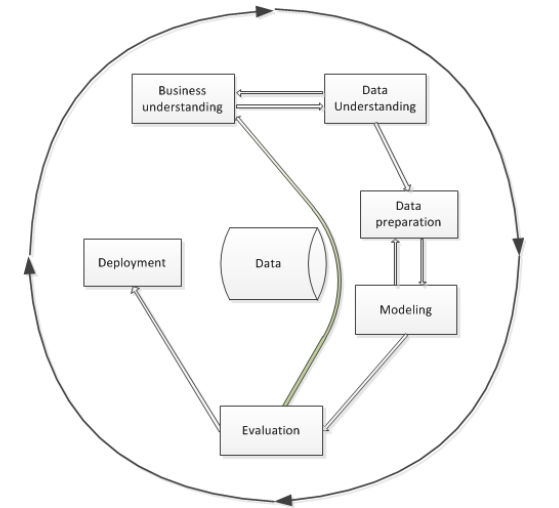
\includegraphics[width=0.85\textwidth]{images/gambarI.2.png}
\caption{Tahapan model referensi CRISP-DM \parencite{niaksu2015}}
\label{fig:I.2}
\end{figure}

\begin{enumerate}
    \item \textbf{Pemahaman Bisnis (\textit{Business Understanding})} \\
    Tahap ini bertujuan untuk mengidentifikasi kebutuhan serta masalah inti yang ingin diselesaikan melalui pemanfaatan data. Dalam konteks penelitian ini, permasalahan yang diangkat adalah ketidaktepatan jawaban teknis yang dihasilkan \textit{Large Language Models} (LLM) ketika merujuk dokumentasi Kubernetes, terutama pada konfigurasi YAML yang bersifat struktural dan rentan mengandung halusinasi. Oleh karena itu, kebutuhan penelitian diarahkan pada peningkatan akurasi penalaran struktural pada proses \textit{retrieval} serta mitigasi halusinasi konfigurasi pada sistem \textit{cloud-native}.

    \item \textbf{Pemahaman Data (\textit{Data Understanding})} \\
    Fase ini berfokus pada pengumpulan dan eksplorasi sumber data untuk memahami struktur, kualitas, serta batasannya. Pada penelitian ini, data diperoleh dari spesifikasi resmi Kubernetes OpenAPI yang dianalisis untuk memahami jenis objek Kubernetes, atribut yang dimiliki, serta relasi hierarkis dan referensial antar-objek Kubernetes. Pemahaman ini menentukan objek Kubernetes yang akan dimodelkan dalam \textit{knowledge graph}.

    \item \textbf{Persiapan Data (\textit{Data Preparation})} \\
    Tahapan ini mencakup pembersihan dan transformasi data agar siap digunakan dalam proses pemodelan. Dalam penelitian ini, dilakukan ekstraksi berbasis \textit{script} dari spesifikasi OpenAPI Kubernetes (JSON) untuk membentuk representasi entitas, yaitu relasi yang dapat dimodelkan sebagai \textit{Knowledge Graph}. Proses ini mencakup identifikasi objek, pemetaan hubungan antar-objek, serta penghubungan \textit{cross-resource references}. Hasil akhirnya berupa struktur graf yang siap digunakan pada mekanisme \textit{retrieval}.

    \item \textbf{Pemodelan (\textit{Modeling})} \\
    Fase ini bertujuan untuk menerapkan algoritma yang sesuai guna menyelesaikan masalah yang telah dirumuskan. Pada penelitian ini, dibangun mekanisme \textit{graph-guided retrieval} yang menelusuri graf menggunakan \textit{graph traversal} berdasarkan kueri pengguna dan menghasilkan \textit{reasoning path}. Jalur penalaran tersebut kemudian diinjeksikan sebagai konteks pada proses RAG untuk memandu LLM dalam menghasilkan jawaban serta konfigurasi YAML yang sesuai dengan logika sistem Kubernetes.

    \item \textbf{Evaluasi (\textit{Evaluation})} \\
    Tahap evaluasi bertujuan menilai kualitas model dan membandingkannya dengan pendekatan alternatif menggunakan metrik yang terukur. Dalam penelitian ini, kinerja sistem dievaluasi menggunakan metrik \textit{answer quality}, \textit{retrieval quality}, dan \textit{reasoning quality}, kemudian dibandingkan dengan dua \textit{baseline}, yaitu \textit{Vanilla LLM} dan \textit{Vector-based RAG}.

    \item \textbf{Penyebaran (\textit{Deployment})} \\
    Fase ini berkaitan dengan penyajian hasil implementasi dalam bentuk prototipe dan dokumentasi. Pada penelitian ini, penyebaran diwujudkan dalam bentuk antarmuka web interaktif berbasis Streamlit yang menampilkan jawaban, konfigurasi YAML, serta \textit{reasoning path} sebagai bukti penalaran graf. Selain itu, dokumentasi lengkap disusun sebagai bentuk penyebaran akademik yang memuat rancangan sistem, hasil evaluasi, serta rekomendasi penelitian selanjutnya.
\end{enumerate}